%%
%% This is file `sample-acmlarge.tex',
%% generated with the docstrip utility.
%%
%% The original source files were:
%%
%% samples.dtx  (with options: `all,journal,bibtex,acmlarge')
%% 
%% IMPORTANT NOTICE:
%% 
%% For the copyright see the source file.
%% 
%% Any modified versions of this file must be renamed
%% with new filenames distinct from sample-acmlarge.tex.
%% 
%% For distribution of the original source see the terms
%% for copying and modification in the file samples.dtx.
%% 
%% This generated file may be distributed as long as the
%% original source files, as listed above, are part of the
%% same distribution. (The sources need not necessarily be
%% in the same archive or directory.)
%%
%%
%% Commands for TeXCount
%TC:macro \cite [option:text,text]
%TC:macro \citep [option:text,text]
%TC:macro \citet [option:text,text]
%TC:envir table 0 1
%TC:envir table* 0 1
%TC:envir tabular [ignore] word
%TC:envir displaymath 0 word
%TC:envir math 0 word
%TC:envir comment 0 0
%%
%% The first command in your LaTeX source must be the \documentclass
%% command.
%%
%% For submission and review of your manuscript please change the
%% command to \documentclass[manuscript, screen, review]{acmart}.
%%
%% When submitting camera ready or to TAPS, please change the command
%% to \documentclass[sigconf]{acmart} or whichever template is required
%% for your publication.
%%
%%
\documentclass[acmlarge]{acmart}

\setcopyright{none}             % No ACM copyright footer
\acmYear{2025}
\acmConference[CHI Project]{CHI-style HCI Class Project}{April 2025}{Colorado State University}
\acmBooktitle{CHI-style HCI Class Project (April 2025, Colorado State University)}
\acmPrice{0.00}
\acmDOI{}                       % Leave empty for assignments
\acmISBN{}   
\usepackage{graphicx}  % Required to insert images % Leave empty
\usepackage{subcaption}
\usepackage{float}



%%
%% \BibTeX command to typeset BibTeX logo in the docs
\AtBeginDocument{%
  \providecommand\BibTeX{{%
    Bib\TeX}}}

%%
%% Submission ID.
%% Use this when submitting an article to a sponsored event. You'll
%% receive a unique submission ID from the organizers
%% of the event, and this ID should be used as the parameter to this command.
%%\acmSubmissionID{123-A56-BU3}

%%
%% For managing citations, it is recommended to use bibliography
%% files in BibTeX format.
%%
%% You can then either use BibTeX with the ACM-Reference-Format style,
%% or BibLaTeX with the acmnumeric or acmauthoryear sytles, that include
%% support for advanced citation of software artefact from the
%% biblatex-software package, also separately available on CTAN.
%%
%% Look at the sample-*-biblatex.tex files for templates showcasing
%% the biblatex styles.
%%

%%
%% The majority of ACM publications use numbered citations and
%% references.  The command \citestyle{authoryear} switches to the
%% "author year" style.
%%
%% If you are preparing content for an event
%% sponsored by ACM SIGGRAPH, you must use the "author year" style of
%% citations and references.
%% Uncommenting
%% the next command will enable that style.
%%\citestyle{acmauthoryear}
%%
%% end of the preamble, start of the body of the document source.
\begin{document}

%%
%% The "title" command has an optional parameter,
%% allowing the author to define a "short title" to be used in page headers.

%%
%% The "author" command and its associated commands are used to define
%% the authors and their affiliations.
%% Of note is the shared affiliation of the first two authors, and the
%% "authornote" and "authornotemark" commands
%% used to denote shared contribution to the research.

\title[Look, Type, Repeat]{Look, Type, Repeat: Measuring Typing Performance Across Visual and Physical Interfaces in VR}

\author{Ben Harper}
\affiliation{%
  \institution{Colorado State University}
  \country{USA}}
\email{benharpr@colostate.edu}

\author{Mack Ianni}
\affiliation{%
  \institution{Colorado State University}
  \country{USA}}
\email{mack.ianni@colostate.edu}

\author{Jovani Reyes}
\affiliation{%
  \institution{Colorado State University}
  \country{USA}}
\email{jovani.reyes@colostate.edu}

\renewcommand{\shortauthors}{Jovani Reyes, Ben Harper, Mack Ianni}


%%
%% By default, the full list of authors will be used in the page
%% headers. Often, this list is too long, and will overlap
%% other information printed in the page headers. This command allows
%% the author to define a more concise list
%% of authors' names for this purpose.
\renewcommand{\shortauthors}{Reyes, Ianni, and Harper}

%%
%% The abstract is a short summary of the work to be presented in the
%% article.
\begin{abstract}
In this paper, we investigate why typing in VR is measurably slower than in traditional computing setups, and how visual feedback and input modalities contribute to this gap in performance. Through this work, we aim to understand whether or not visual cues or differing modalities aid or impact performance. In our experiment, participants typed under three separate conditions: a traditional desktop and keyboard setup, with a monitor inside a first-person game world, a virtual reality environment with head-mounted display, physical keyboard, hands displayed, and lastly a virtual reality environment with a head-mounted display, physical keyboard input, with hands not displayed. Additionally, we looked into methods such as virtual keyboard typing, with hands toggled on and off, but ultimately ran into too many technological limitations when accounting for simulating key presses with the MetaXR hand tracking. As a result, we will mainly explore our experimental conditions, and then touch on the virtual typing with a virtual keyboard in our future work and limitations. Overall, there is a significant drop in typing performance when visual feedback is removed in the virtual world, and from our study, participants noted that the desktop and keyboard in the game world was clearly the best, but interestingly enough it was also stated that in the virtual environment, the virtual hands made it harder to type and to see. 
\end{abstract}

%%
%% The code below is generated by the tool at http://dl.acm.org/ccs.cfm.
%% Please copy and paste the code instead of the example below.
%%
\begin{CCSXML}
<ccs2012>
 <concept>
  <concept_id>10003120.10003121.10003125</concept_id>
  <concept_desc>Human-centered computing~Text input</concept_desc>
  <concept_significance>500</concept_significance>
 </concept>
 <concept>
  <concept_id>10003120.10003121.10003124</concept_id>
  <concept_desc>Human-centered computing~Interaction devices</concept_desc>
  <concept_significance>500</concept_significance>
 </concept>
 <concept>
  <concept_id>10003120.10003121.10011748</concept_id>
  <concept_desc>Human-centered computing~Virtual reality</concept_desc>
  <concept_significance>500</concept_significance>
 </concept>
 <concept>
  <concept_id>10003120.10003145.10003146</concept_id>
  <concept_desc>Human-centered computing~User studies</concept_desc>
  <concept_significance>500</concept_significance>
 </concept>
</ccs2012>
\end{CCSXML}

\ccsdesc[500]{Human-centered computing~Text input}  
\ccsdesc[500]{Human-centered computing~Interaction devices}  
\ccsdesc[500]{Human-centered computing~Virtual reality}  
\ccsdesc[500]{Human-centered computing~User studies}  


%%
%% Keywords. The author(s) should pick words that accurately describe
%% the work being presented. Separate the keywords with commas.
\keywords{Text entry; virtual reality; hand visualization; physical keyboard; human-computer interaction; typing performance; immersive environments; head-mounted display; input techniques; user study}


%%
%% This command processes the author and affiliation and title
%% information and builds the first part of the formatted document.
\maketitle

\section{Introduction}
In today's day and age, typing is arguably one of the most important tasks that humans do on a day-to-day basis. Typing allows humans to transfer their thoughts and ideas into beautiful creations, which aids in work, education, learning, gaming, coding, and more. Over the last 10 or so years, with the world's increasing digitization, many people have become more interested in spending their time in virtual worlds, similar to the movie \textit{Ready Player One}. As more virtual environments are explored, there is an increasing demand for highly responsive and accurate text input. An increase in accuracy, precision, and speed would be required if we wanted to integrate these augmented or virtual reality systems into workspaces, classrooms, research labs, and other environments. However, despite all of the advances across the extended reality continuum in hand tracking and other hardware, text input in VR is still slow and inaccurate, remaining significantly slower and more error-prone than in traditional desktop environments~\cite{Son2019}. A large part of this performance gap comes from the fact that wearing a head-mounted display (HMD) reduces the user's awareness of their environment and sense of body awareness when compared to the real world. This is because when one is wearing the HMD they typically cannot see their physical hands, fingers, or other real-world objects while inside the virtual environment. 

Beyond traditional keyboard and monitor virtual reality typing setups, other text input interaction methods have been studied over the years. Interaction methods such as two thumb typing with handheld controllers, proposed by Son et al.~\cite{Son2019}, demonstrated that visual feedback such as hovering thumbs increased performance with users reaching up to 30 WPM after brief training. Findings like these reinforce the importance of visual and motor alignment when working in immersive environments. While previous research has investigated physical keyboards with and without hand feedback~\cite{Knierim2018}, or controller-based virtual keyboards~\cite{Boletsis2019, Dudley2019}, our research aims to show specifically the impact of virtual hands, as well as the impact of wearing an HMD.

This research investigates how typing speed and performance are affected in virtual reality across three conditions to validate our thesis, and to learn more about the area. Our conditions are (1) a traditional desktop setup with a physical keyboard inside an Unreal Engine game environment, (2) a VR environment with a physical keyboard and virtual hand visualization, and (3) a VR environment with a physical keyboard and no virtual hand visualization. While we originally proposed an additional input method of a fully virtual keyboard, it proved infeasible due to the limitations of hand tracking from only a headset.



\section{Related Work}

Physical keyboard text input is crucial for everyday life, with 98\% of surveyed medical residents saying that it is at least somewhat important to their careers~\cite{Kalava2014}. Virtual reality systems have also seen an increase in usage and development, with 77 million users in 2024 expected to grow to 91.3 million in 2028~\cite{Kumar2024}. Despite the importance of text entry and the increasing adoption of virtual reality, there are still many issues in the realm of keyboard text input inside virtual reality systems~\cite{Speicher2018}. Here we introduce and review common methods and recent developments for text input methods in virtual reality environments. We examine studies involving physical keyboards in VR, then consider alternative input approaches including virtual keyboards and controller-based methods.



\subsection{Physical Keyboard Text Input In VR}

Physical keyboard text input in virtual reality systems aims to leverage the benefits that typing has in the real world by combining a physical keyboard and the virtual environment, or a virtual keyboard that a user may type on. In the case of a physical keyboard in a virtual environment, the user will suffer from not being able to know the exact position of their hands, and may also struggle with misalignment of the physical keyboard and its virtual representation. In the case of a virtual keyboard, the user may struggle from inaccurate hand tracking. Both of these cases might cause worse performance compared to real world typing. Knierim et al. highlighted this when he demonstrated that typing performance for inexperienced users using a physical keyboard in VR dropped when compared to real-world input, reporting an average of 31.8 WPM in VR without hand visualization versus 45.4 WPM in the real world~\cite{Knierim2018}. Another study by Grubert et al. explored typing in VR with desktop and touchscreen keyboards, reporting speeds from 26.3 WPM for desktop keyboards and only 11.6 WPM for touchscreen keyboards in VR, compared to 41.4 WPM and 24.0 WPM from outside of the VR environment, finding that users retain around 60 percent of their physical world typing speed~\cite{Grubert2018}. With very intricate and advanced technology, such as sensors on keyboards and exact visualizations of the keyboard, Walker et al. reported that users typed at 41.2 WPM in VR using a physical keyboard, and 43.7 WPM when a virtual assistant visualized key press feedback~\cite{Walker2017}. This was outstanding, but the results were still much slower than the desktop baseline of 60 WPM, indicating that hand feedback aided typing is still slower than the real world typing. Furthermore, Chellali et al. supported this claim by demonstrating how keypress visual feedback significantly improved typing speed ($F(1,21) = 16.99$, $p < .0001$, $\eta^2 = .44$) and reduced cognitive workload (p = .002), while hover feedback reduced error rates (p = .004)~\cite{Chellali2025}. However, using a physical keyboard for passive haptic feedback increased error rates (p = .02), likely due to spatial misalignment between virtual and physical keys.




\subsection{Virtual Keyboard Typing Text Input in VR}

In a perfect world, virtual keyboard typing in VR environments would be as easy as it is typing on a physical keyboard, but this is not the case. As a result, tons of research and studies have been conducted to evaluate the best methods of typing virtually in the VR environments to achieve the same usability and speed as a normal keyboard and display. Many studies have articulated the fact that there are many limitations in this area, such as positioning limitations, the occlusion of one's hands, fatigue issues when typing, and lack of tactile feedback in the environments. Kim et al. demonstrated in their research that key size and spacing in virtual keyboards significantly influence a typist's output and mental/physical strain, which suggests that having an accurate design and representation of the keyboard in virtual reality is key to achieving the best results.~\cite{Kim2013}. More experimental methods have been tested to potentially solve this issue as well. Boletsis and Chorianopoulos compared four controller-based techniques: ray-casting (16.65 WPM), a drum-like keyboard (21.01 WPM), head-directed input (10.83 WPM) and a split keyboard (10.17 WPM), finding that even the fastest method, the drum-like keyboard, still is not even close to traditional typing speeds (40-60 WPM)~\cite{Boletsis2019}. Work done by Foy et al. highlighted the differences between two-finger and ten-finger typing. Typing with two fingers on a surface yielded the highest performance (55.6 WPM), while ten-finger mid-air typing was the slowest and yielded the most errors. Foy also highlighted that ten finger typing suffers from accidental key presses quite often and it makes it much more difficult to use compared to the two-finger typing~\cite{Foy2021}. Their work reinforces the findings that without decoders or tactile support, purely virtual input strategies become highly error prone, which is what we had experienced when we attempted to create our own version of a virtual keyboard with ten-finger typing. The lower speeds in these environments are attributed to the variables in the virtual environments listed earlier. Due to the success of Walker et al. we attempted to implement our own version of a virtual keyboard representation that included contact pivots at the fingertips, but, we were ultimately unsuccessful in creating an experiment usable environment, given time constraints. Due to this, we figured that we would follow Dudley et al. who claimed the best results have come from when the virtual keyboard is aligned in conjunction with a physical surface. In their study, they evaluated four VR text entry strategies and found that virtual keyboards aligned with a physical surface significantly outperformed mid-air alternatives~\cite{Dudley2019}. There has also been interesting work done on text entry techniques that reduce the usage of the user's hands, such as using gaze to assist with typing. Zhao et al. developed two strategies for typing in mid-air that significantly reduced the movement required for a given input~\cite{Zhao2023}, which could help in solving the issue of exhaustion from a user holding their hands out in front of them. Several other studies have attempted methods that do not involve the user's hands whatsoever, which do reduce the strain on the user's hands~\cite{Rajanna2018, Hu2024}. However, methods that rely only on gaze generally suffer from much lower speeds than typing based approaches, with even an approach that claims speed as one of its key advantages achieving average speeds of only 15.42 WPM~\cite{Hu2024}, compared to a physical keyboard's average of 40-60 WPM.

\subsection{Hand Visualization Aiding Text Input in VR}

Hand visualization in VR environments has long been discussed as to whether it helps or harms VR typing performance. One theory posits that if the user is able to see their hands and fingers in the environment, they will feel more immersed, leading to better results. Typically, the hands are not able to be seen due to the user wearing a head-mounted display. Grubert et al. demonstrated the importance of hand and fingertip visualization when they reported that fingertip visualization reduces error rates and slightly increases speeds (29.2 to 29.5 words per minute vs. 26.4 words per minute without hands). They also noted that experienced typists achieve almost the same level of performance as a normal keyboard, which was close to 45.9 words per minute ~\cite{Grubert2018}. On the other hand, inexperienced typists achieved only 40 words per minute. Both words per minute rates were achieved using semi-transparent hands in the environment.  ~\cite{Walker2017} Zhang et al. investigated five different hand representations that varied in terms of realism, which suggested that hand visualization helps bridge the performance gaps that occur in virtual reality systems, especially for beginner and intermediate typists. Zhang et al. found that hand realism and hand presence influences the user's sense of perception, ownership, and immersion in VR~\cite{Zhang2020}. In a questionnaire, users rated the realistic hands higher in presence compared to the block hands or cursor hands.(17.93 vs. 15.62, with a p value of 0.001) In another study, Giovannelli et al. found that even when hands were exposed for a short period of time subjects hesitated less when typing and their typing speed was higher.~\cite{Giovannelli2022} Similarly, Zaman et al. emphasized how when the user sees their hands, their sensory receptors respond better, reducing fatigue and mental effort of the user ~\cite{Zaman2022}. The same finding was also demonstrated by Lougiakis et al., who showed that when hands are represented well in virtual reality it increases the user's sense of ownership over the hands~\cite{Lougiakis2020}. On the other side, Venkatakrishnan et al noted that the use of physical controllers combined with hand visualizations can have negative effects on performance, and recommended the use of other hand tracking methods such as gloves.~\cite{Venkatakrishnan2023}.

\section{Methodology}

For our study, we wanted to test the relationship and importance of virtual hands in the virtual environment and the subjects' ability to perform typing tasks in the environment with and without hands displayed. Our Unreal Engine world also included a baseline where the subject is in a first-person game, typing on a monitor as one would in a traditional computing setup. Words per minute, error rate, average time to complete the tasks, character error rate, and accuracy were tracked during the experiments. We made sure to run the baseline condition first so that the subject could warm up on the keyboard, and then later had the subject put on the head-mounted display and enter the virtual environment, where a randomly generated sequence occurs that starts a subject in the environment with their hands either visible or invisible. The user would complete 10 typing tasks for each experimental condition to the best of their ability in the order determined by the game world. Subjects were notified on the screen if they had pressed an incorrect key, with feedback appearing on the monitor where the subject would type the words. The physical keyboard that was simulated in the virtual world also had feedback on the key input that simulated a key press, but the keys did not light up or do anything tactile other than that.

% Add this right before \section{Methodology}
% Add this right before \section{Methodology}
\begin{figure}[H]
    \centering
    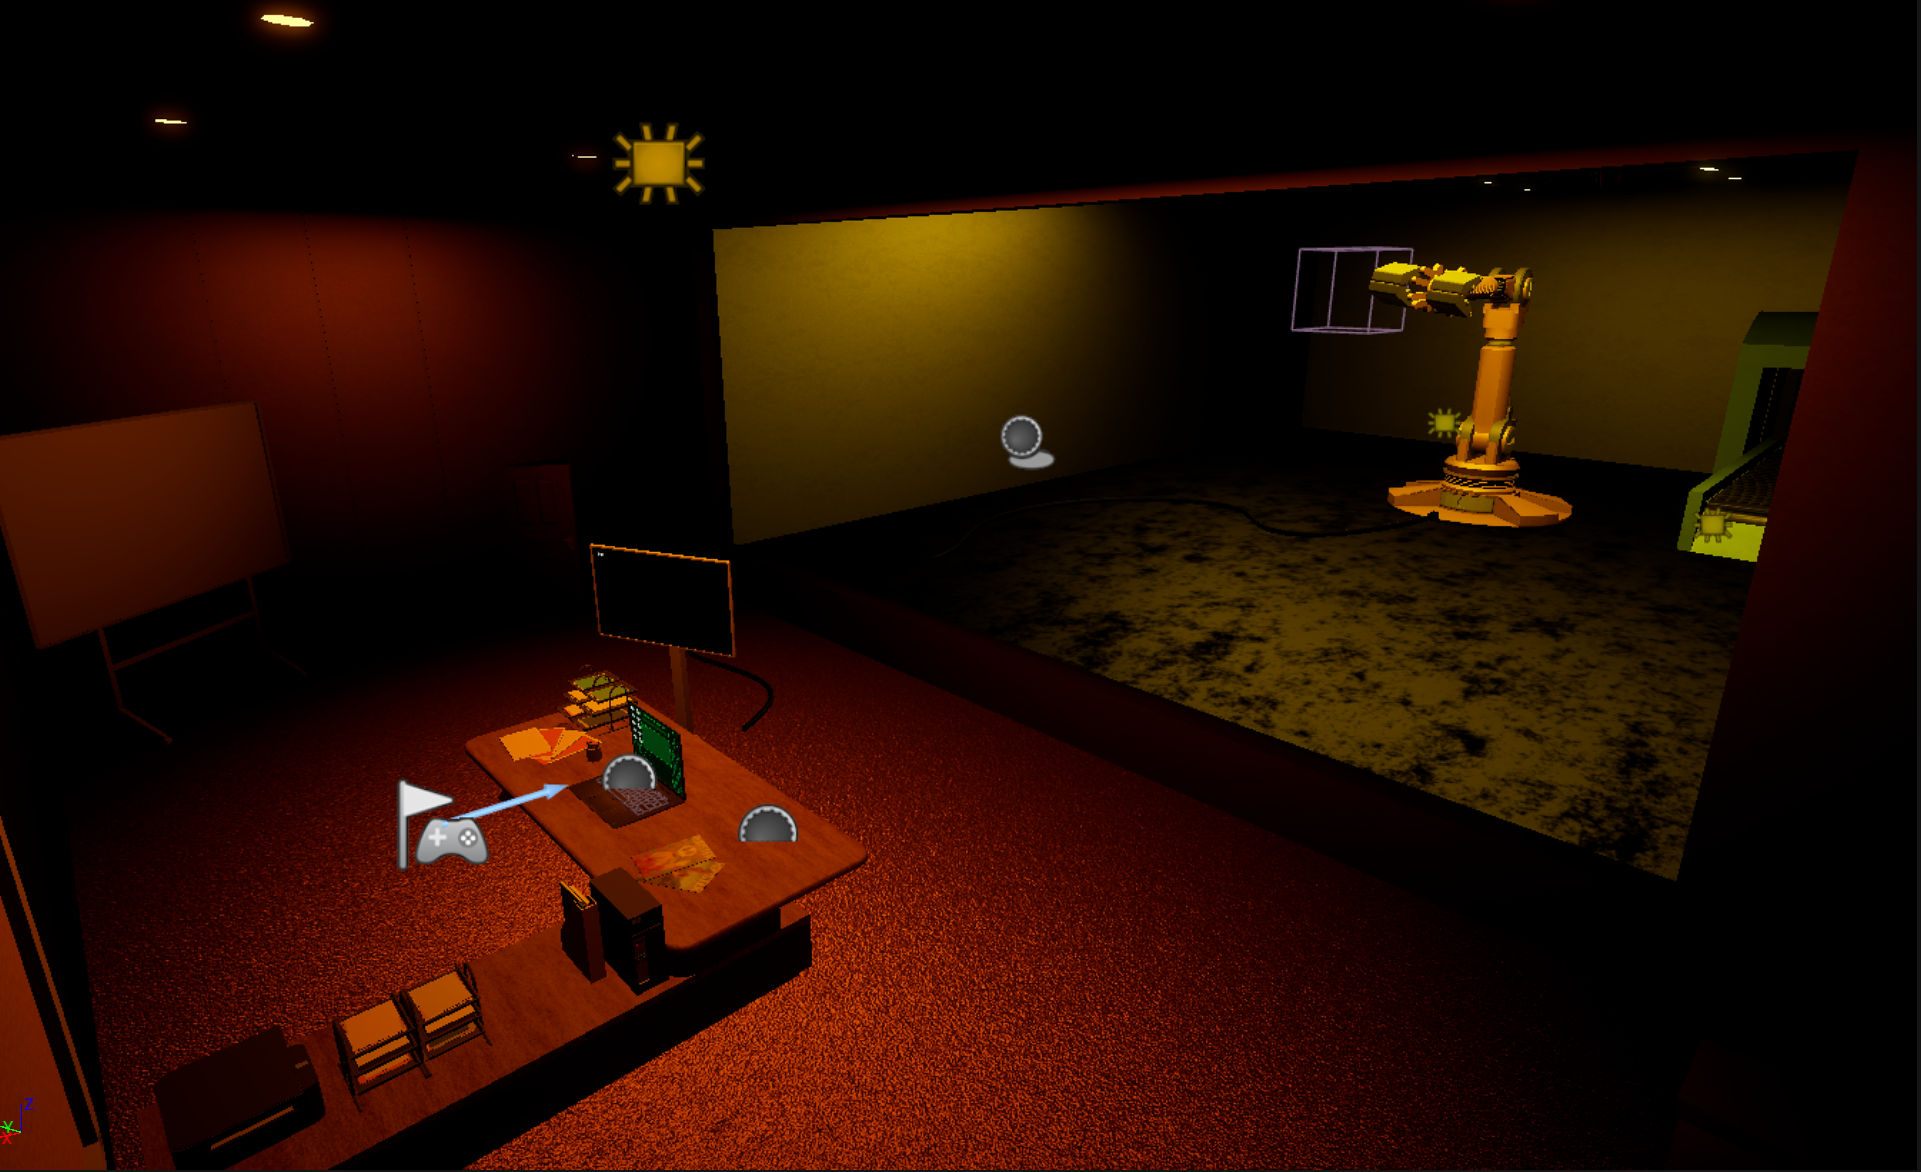
\includegraphics[height=4.5cm]{world_image.png}
    \caption{Virtual lab environment where participants interacted with the experimental interface and robotic system.}
    \label{fig:world_environment}
\end{figure}



\subsection{Participants}

The participants in our experiment go to Colorado State University between the ages of 20 and 24. Most of the participants were recruited from the CS465 teams channel, while other participants were friends of ours. Before starting the experiment, participants first completed a survey so that we could collect their demographic information. This survey was created to capture age, gender, handedness, typing proficiency, and prior VR experience. In addition, participants were asked how often they type using a keyboard, VR usage, and whether or not they have tried keyboard or text input in a virtual reality environment. Most of the participants reported regular keyboard use, while others reported that they only typed when they needed to. The participants then completed each experimental condition, with a break offered after each. After the experiment, we had them answer another qualitative survey. This survey asked to rate their perceived comfort between the baseline, the virtual head-mounted display with hands displayed, and the virtual head-mounted display typing with no hands displayed. This was ranked from one being very uncomfortable, to five very comfortable. 91.7 percent of our participants were aged 22–23, with last 8.3 percent being ages 20–21. 91.7 percent of the participants were male, while only 8.3 percent were female. 75 percent of participants stated they use keyboards to type daily, while 25 percent said they use a keyboard multiple times per day. 50 percent of participants said that they sometimes have to look at the keyboard, whereas 41.7 percent said that they do not have to look at the keyboard, and 8.3 percent said that they have to look at the keyboard when they type all of the time. When asked about their virtual reality experience, 41.7 percent of participants stated that they have somewhat used VR, 33.3 percent said they rarely have used it, and 25 percent have used it extensively. Lastly, a majority of the participants have never used VR with a head-mounted display and keyboard. They were then asked what they thought were the two most accurate methods of key input and their self-identified typing speed e.g. “slow” or “very fast”. We then collected some more qualitative questions such as asking which interface was the most frustrating to use, challenges, and something that they would change about our experiment. Participants were thanked for their time and help and went on their way. 


\subsection{Design}

This study used a "within subjects" method in which each participant completed the three typing conditions. While we had originally planned to balance the order of the experimental conditions, we concluded that allowing subjects to perform the baseline first would allow us better insight into the comparison between typing speeds with and without hand visualization.


The three conditions were selected to isolate the effects of physical input versus visual feedback.


\begin{enumerate}
    \item \textbf{Desktop Baseline (No VR)}  
    
    Participants typed on a traditional physical QWERTY keyboard while viewing a standard desktop monitor in Unreal Engine. Hands were visible naturally. This served as the control condition for baseline performance.

    \item \textbf{VR + Physical Keyboard (With Virtual Hands)}  
    
    Participants wore a head-mounted display (HMD) and typed on a physical keyboard. Their hands were rendered as virtual models aligned with their real hand positions to provide immersive typing with tactile feedback and support.

    \item \textbf{VR + Virtual Keyboard (No Physical Keyboard)}  
    
    Participants used tracked virtual hands to type on a virtual keyboard with no physical keys. Input was registered through hand collisions with the virtual keyboard surface. This condition simulates controller-free VR input relying on hand tracking and visual feedback only.
\end{enumerate}

\begin{figure}[htbp]
    \centering

    \begin{subfigure}[t]{0.3\linewidth}
        \centering
        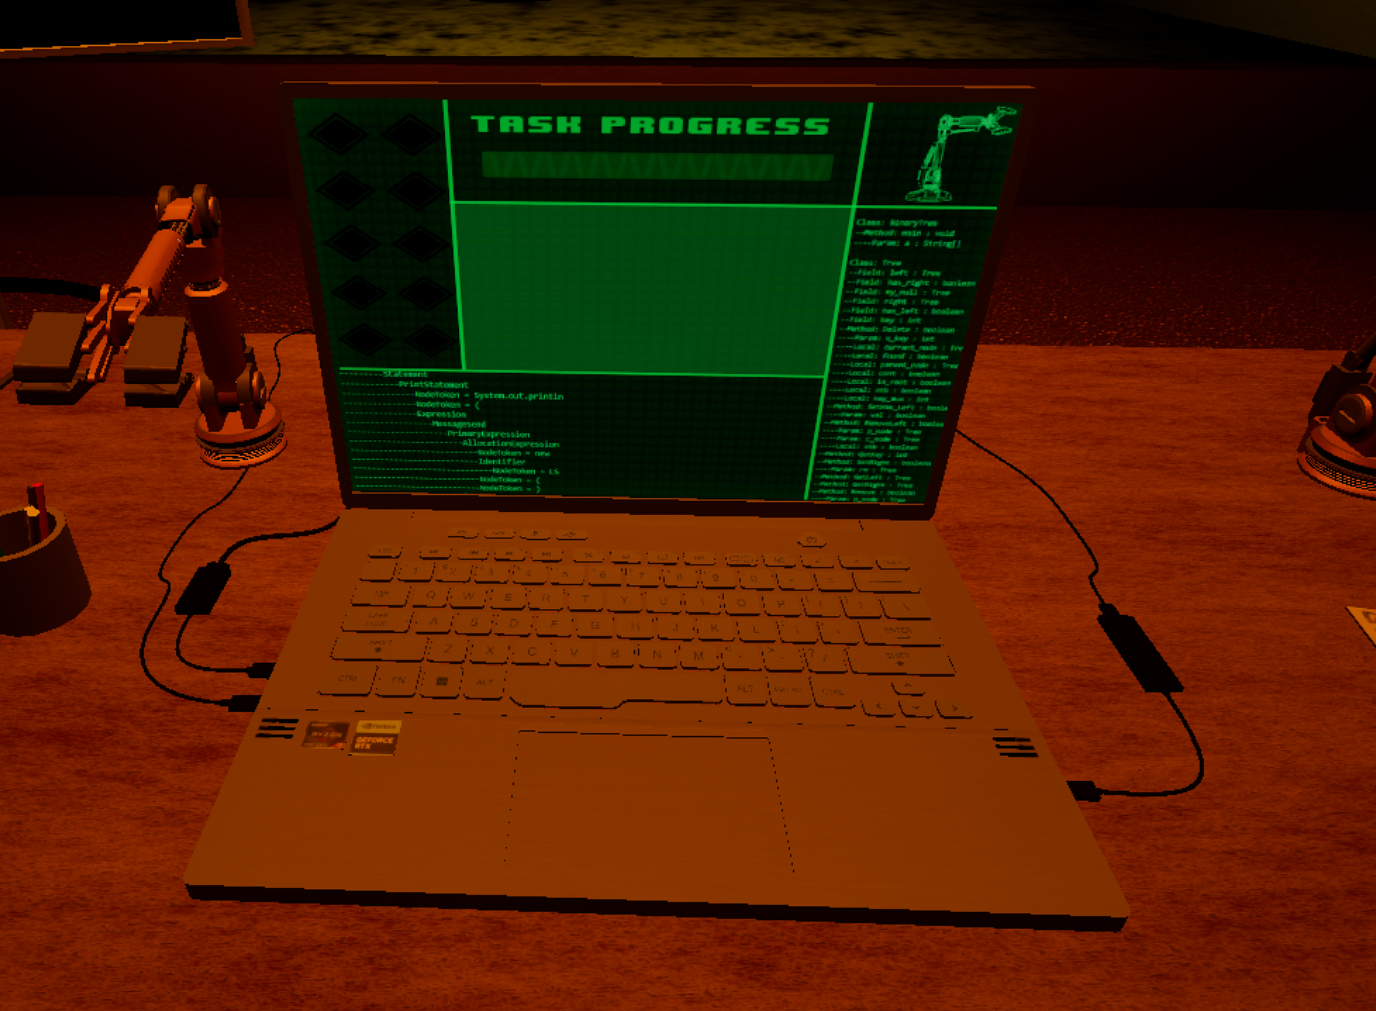
\includegraphics[width=\linewidth]{keyboard3.png}
        \caption{Standard desktop setup with external monitor and full-size keyboard.}
        \label{fig:setup_desktop}
    \end{subfigure}
    \hfill
    \begin{subfigure}[t]{0.3\linewidth}
        \centering
        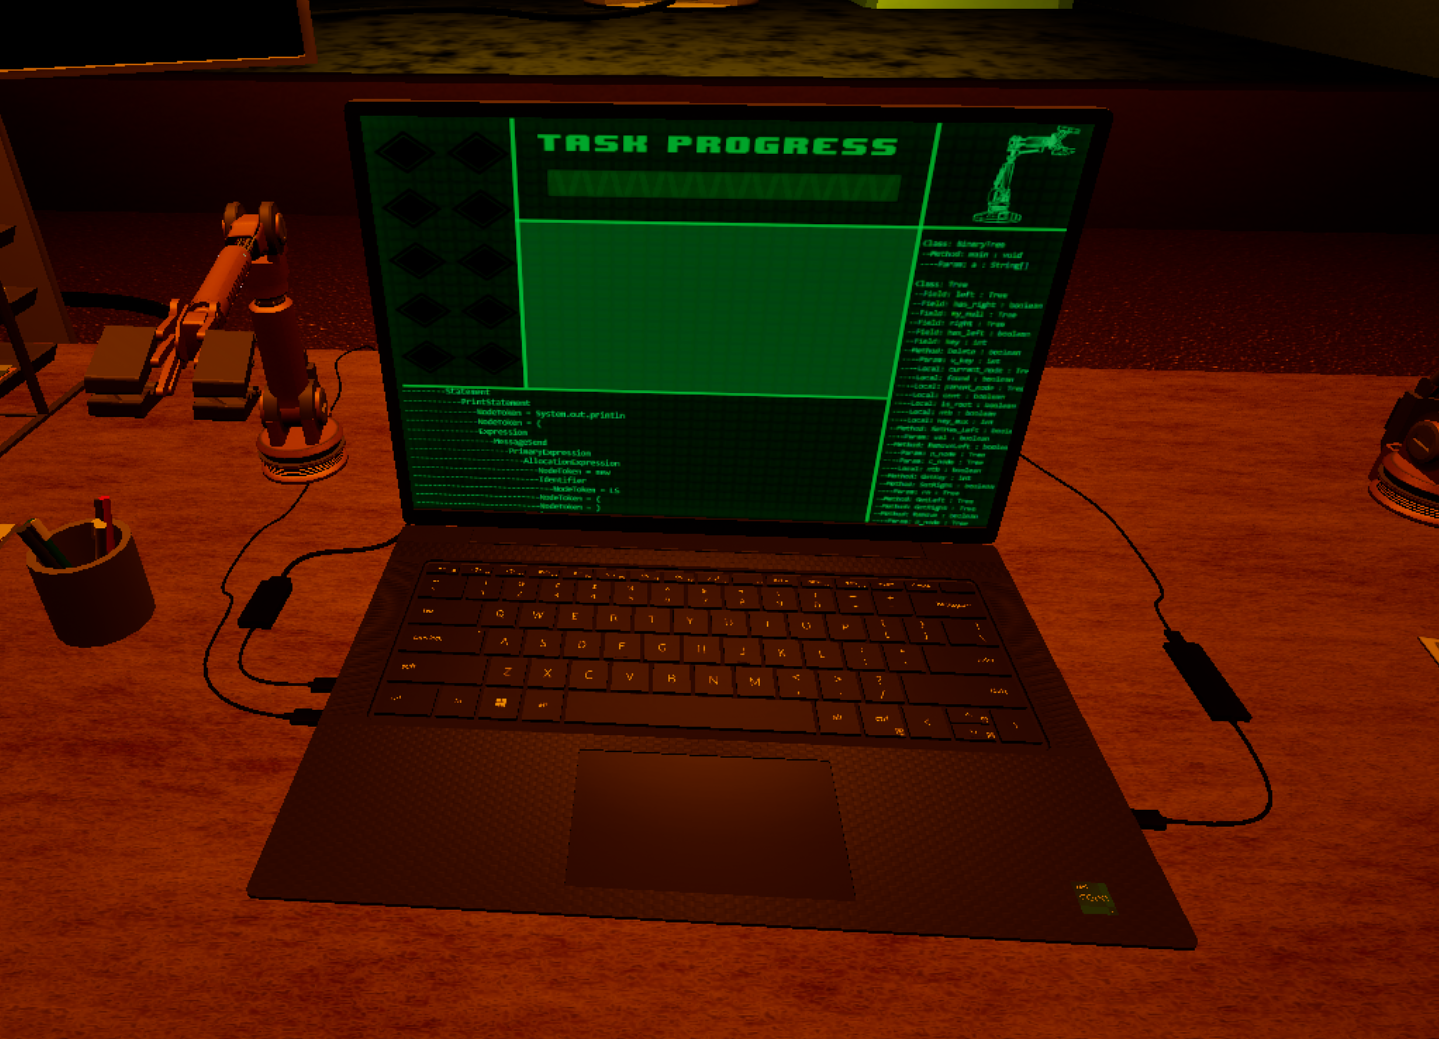
\includegraphics[width=\linewidth]{keyboard1.png}
        \caption{Compact VR-compatible laptop setup used in confined spaces.}
        \label{fig:setup_laptop_black}
    \end{subfigure}
    \hfill
    \begin{subfigure}[t]{0.3\linewidth}
        \centering
        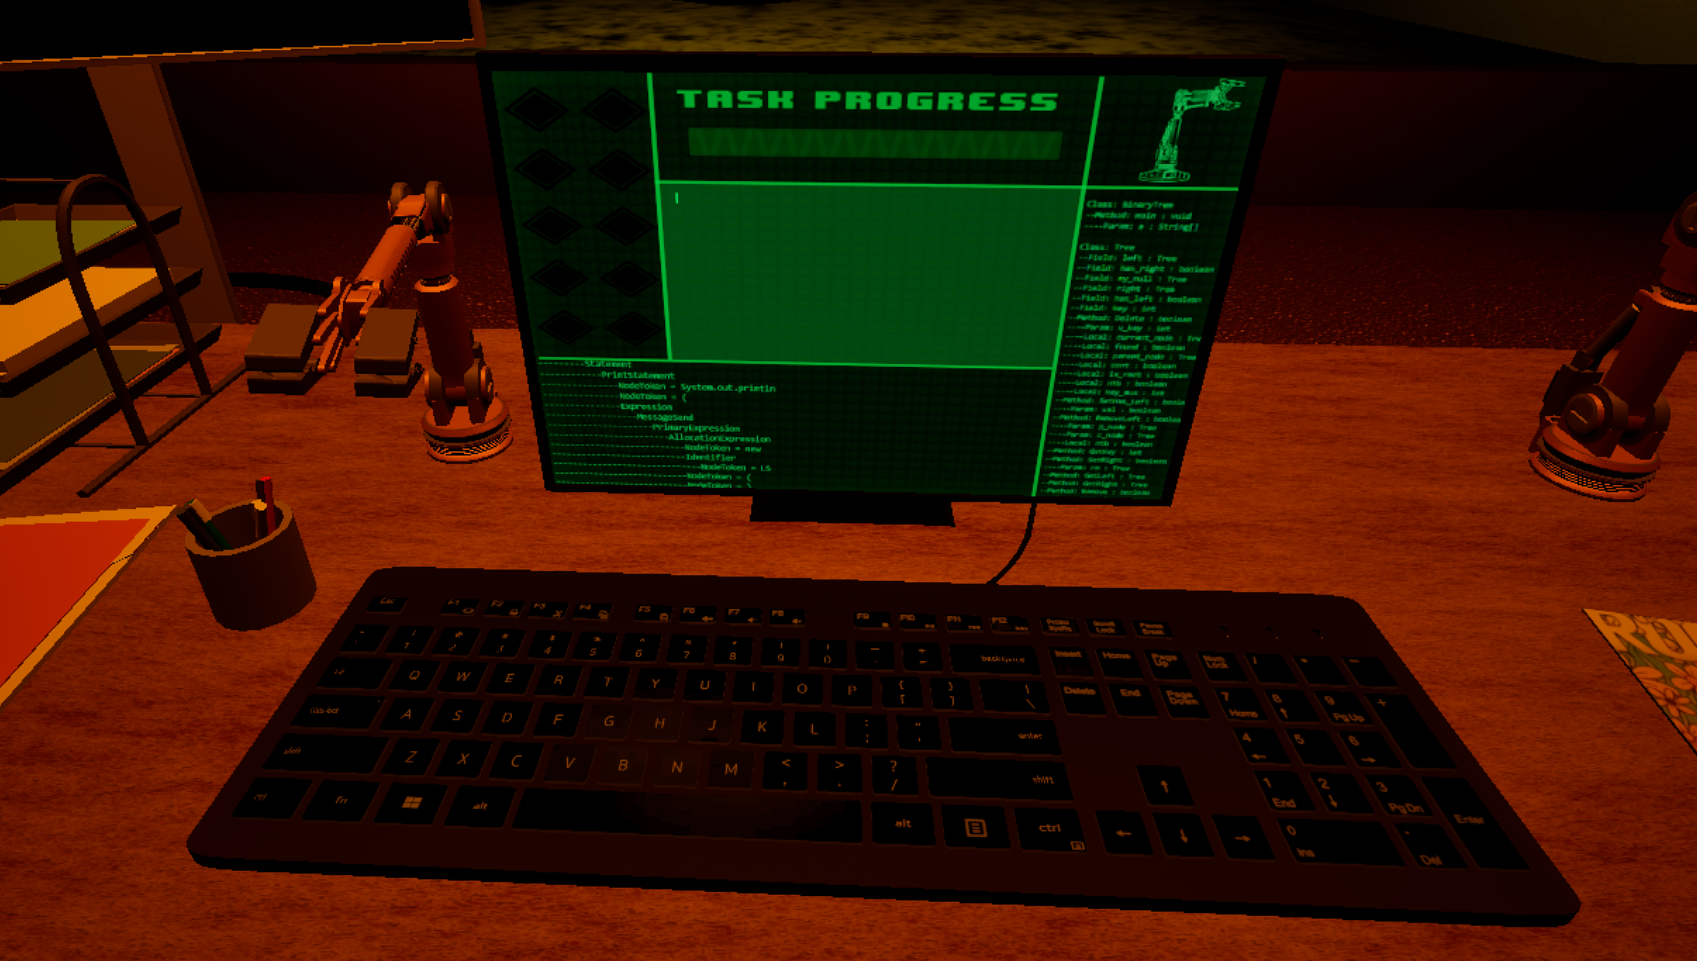
\includegraphics[width=\linewidth]{keyboard2.png}
        \caption{Alternative laptop setup with CS 225 lab keyboard.}
        \label{fig:setup_laptop_white}
    \end{subfigure}

    \caption{Three physical setups used across participants, depending on the experiment location and available workspace. All configurations supported the same software stack and user interface logic.}
    \label{fig:setup_variants}
\end{figure}


\subsection{Apparatus}
% TODO: Describe the system hardware and software, Headings vary (Materials, Interface)
%       Reproductibility extremely important, give all details necessary), use images of the UI

\begin{figure}[htbp]
    \centering

    \begin{subfigure}[t]{0.48\linewidth}
        \centering
        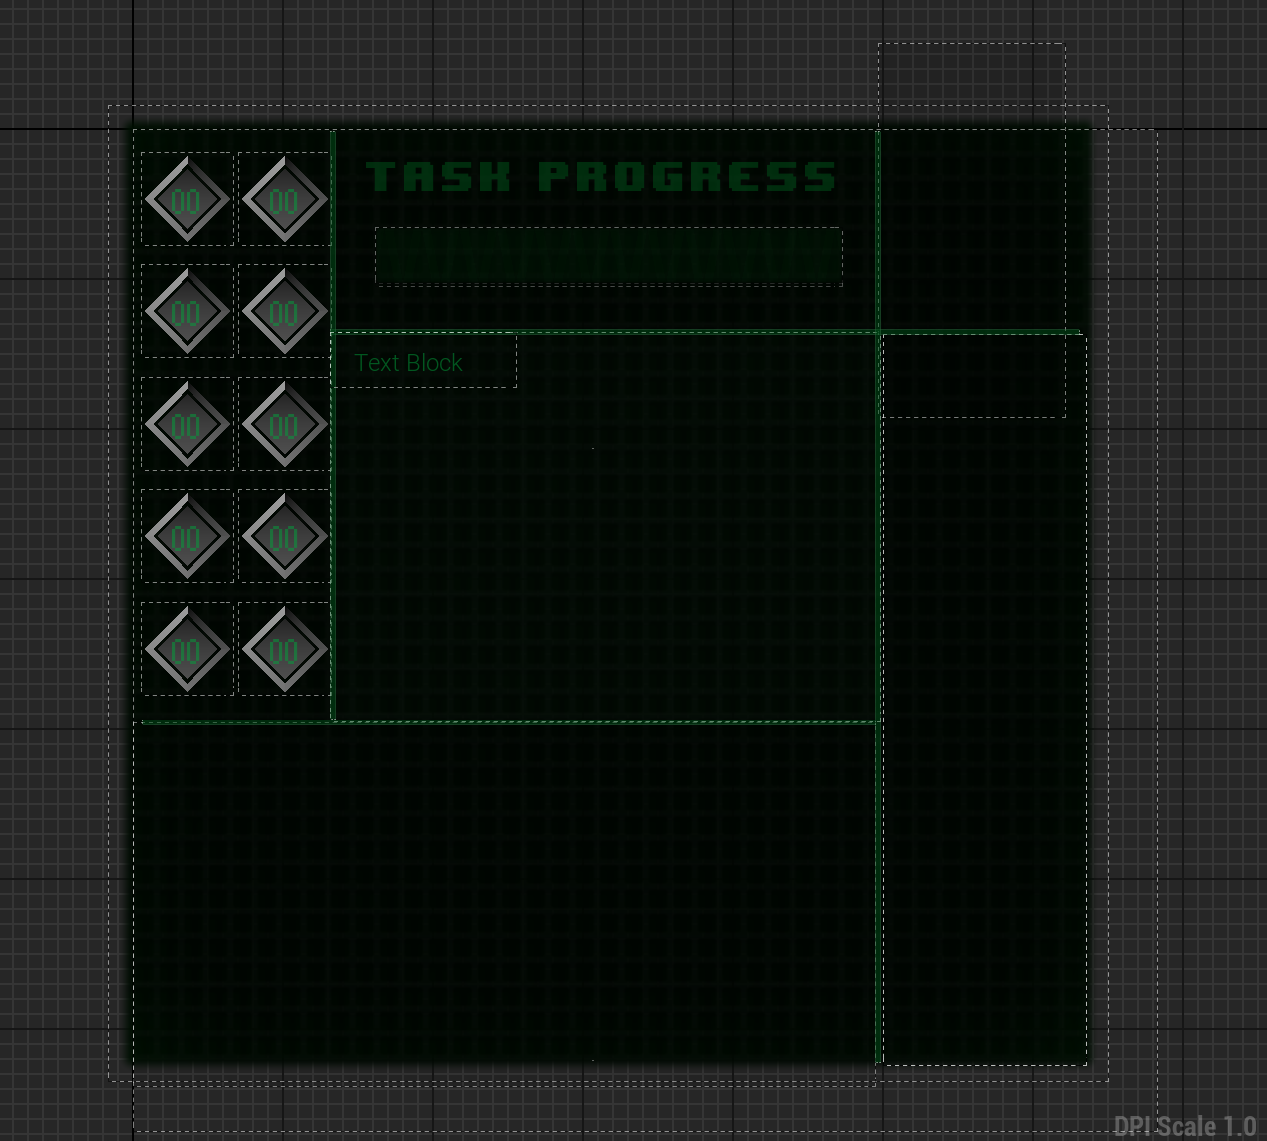
\includegraphics[height=4.5cm]{Monitor_UI.png}
        \caption{UI Blueprint layout in Unreal Engine.}
        \label{fig:monitor_ui}
    \end{subfigure}
    \hfill
    \begin{subfigure}[t]{0.48\linewidth}
        \centering
        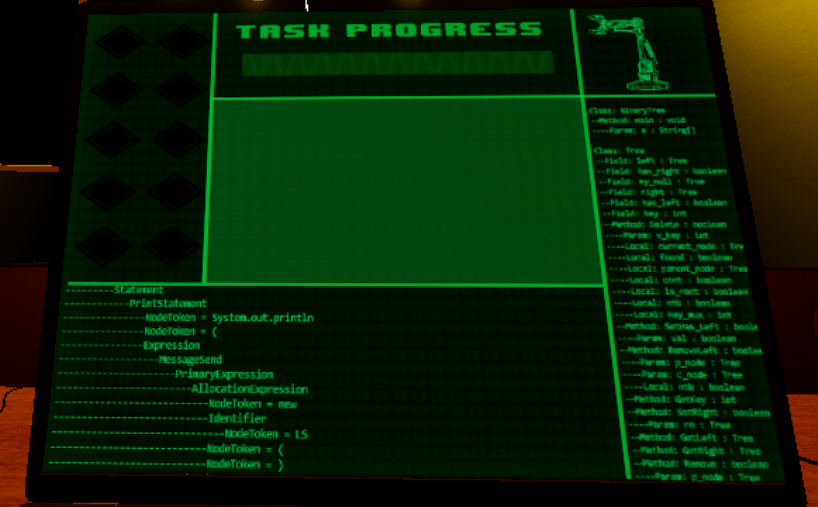
\includegraphics[height=4.5cm]{task_progress.png}
        \caption{In-game display presented to participants.}
        \label{fig:task_progress_render}
    \end{subfigure}

    \caption{UI system design and implementation: (a) layout in Unreal Engine, and (b) rendered interface with real-time feedback.}
    \label{fig:apparatus_ui}
\end{figure}


The study was conducted in the Computer Science Building room 225. All participants were seated at a standard height desk throughout the experiment. To run the experiments, we used a Meta Quest 2 headset and accessories connected to the lab PC. The application was built using Unreal Engine 5.3.2 with Blueprints, and deployed via the Meta Quest Link system for direct PC-VR integration. Virtual hand tracking was implemented using MetaXR hand tracking API kit via the marketplace and was created via blueprint. The virtual keyboard was displayed in front of the participant at a fixed position aligned with their midsection and the keyboard. The physical keyboard used in both the desktop and VR and physical conditions was a standard QWERTY mechanical keyboard (Standard HP Lab Keyboard). For the desktop condition, participants used a standard CSU lab monitor and typed directly into a similar custom full-screen typing interface built in Unreal Engine 5.3.2. The virtual keyboard overlay condition rendered a 3D QWERTY keyboard in VR space. Typing was accomplished by typing on the physical keyboard with the virtual keyboard overlaid. Keystroke events were registered based on collision detection with the physical keyboard. All typing data (words per minute, character error rate, time to complete the task, and accuracy) were logged in real time for later analysis.


\subsection{Reading key presses}
At its root, our implementation for tracking and sanitizing user input on the keyboards relies on the “Any Key” function that is provided through Unreal Engine 5 (UE5) for the physical-input keyboard; and a custom function that reads the name of the key inputs. For every key release and key pressed the name of the key/collision box is checked to be sure that the key is a valid key that we can sanitize and manipulate. 
 
 
\subsection{Storing Key Input}
For every valid key press we append the new character into a string that holds every previous insertion, this string is the text that appears on the UI for the user. The logic for deletion is fairly similar to insertion. For both functions, we either increment or decrement an integer variable to track our current index in the string. This is used to prevent runtime errors if a user attempts to delete more characters than there are available.
 
 
\subsection{Key Pressed}
On a valid key press, the name of the key (i.e. “Q”, “W”, “Backspace”, “Spacebar”) is used to find the unique index value stored in a map[String:Key Name, Int:Index] that correlates with key indexes on a skeletal mesh(The keyboard) which is used for an animation blueprint that sets the z-axis value for that key index downwards from its original location to mimic a real key press. After which the key's name is again used to figure out the type of the key that was pressed(modifier keys such as Ctrl, Shift, or Alt, and action keys like Delete, Enter and alphanumeric keys). A quick solution to separating numeric and letter keys from the modifier and action keys was to simply check if the length of the key name was ‘1’. For alphanumeric keys, we check a Caps Lock flag variable as well an array of key names that are all keys currently being held down, specifically this is done to track left and right Shift key press holds. By checking for Caps Lock and Shift holds, our keyboard successfully handles switching between lower/uppercase as well as displaying symbol characters when shift is held. For Non-alphanumeric keys we handle them case by case depending on what actions need to be done. For Deletion and Backspace we call the function that handles the removal of chars. For Left-Shift, Right-Shift, or Caps Lock a boolean flag is toggled on for the shift keys and for Caps Lock its flag is toggled. For any of these operations, we set a flag to let our function that handles inserting new key inputs know to not append the key since it is not a key meant to be displayed on the UI. 
 
 
\subsection{Key Released} 
When a key is released from the pressed state, we remove it from our string array that holds our keys currently in the pressed state, we also check to see if the key released is the left or right shift key so that its corresponding boolean flag can be turned off. Three flags are used for tracking the state of the shift key, Left-Shift On, Right-Shift On, and Shift-On. Shift-On is evaluated after the first two and is set to true if either one or both of the shift keys are pressed. Lastly, we use the corresponding key index again to set the z-axis of the key back to its initial state. 
 

\subsection{User Interface Widgets}
Currently, there are two monitors displaying UI widgets, the first being used to display the introduction to the project and afterwards, the current task's prompt. The widgets use a Fancy Text Block to dynamically change the color of the text to be White (Default), Green (Right), or Red (Wrong). This feature is the most useful for the users since they can visually see how accurate their input is at each step (currently excluding whitespace). The second UI widget is the user's computer, which includes a text box containing the user's input, a progress bar, and task icons that fill with a color between green (100 percent) and red (0 percent) to display their accuracy as well as the WPM for the task. Other components of the widget are 3 Media textures, the first being a wireframe view of the Claw Bot that loops a rotating view of it, and the other two being code blocks that only play while the user has an Alphanumeric key pressed down. These 3 components are decorative features that are used to stylize the user's UI for a more enjoyable experience. 


\subsection{Calculating WPM and Accuracy}

The timer used to track WPM only begins after the first valid key is pressed for each task in order to mitigate time that shouldn't be measured (i.e. if User 1 sits for 10 seconds during a new task to look around the scene, while User 2 begins instantly, both will have a fair time measurement). Accuracy is checked every time an alphanumeric/symbol key is pressed. The comparison is done by comparing the new input to the character in the prompt  located at the same index (using the index tracker), the boolean value of the comparison is then stored in a dynamically re-sizable boolean array, where each index corresponds to a character in the prompt. After the task is complete, which is checked by comparing the length of the user's string to the length of the prompt; the boolean array is parsed and stores the number of correct and incorrect characters. Accuracy is simply the value of ((Correct) / (Correct + Incorrect)). The value is used in a Lerp function that returns a linear color between green (1.0 Accuracy) and red (0.0 Accuracy). The WPM uses the Net WPM formula in order to account for inaccurate inputs. The resulting integer value of WPM and the Linear Color computed from the accuracy are sent to a function 

\subsection{Storing User data post-runtime}
For storing user data we used a SaveGame Blueprint that is stored in two variables, one for the participant number and the other a map that uses an integer key with a string that contains every task's WPM, Accuracy (1-0), Time (Mins) for task, and every keystroke made including Deletion, Shift, Caps Lock, Spacebar, etc. 
 
In the GlobalVariable blueprint, the variables stored in SaveGame would be checked at the start of every game session, if there existed saved data already on the given filename, then it would be stored within the current session and used at the end of the experiment. So, at the end of the last task, the new user data would be appended to the pre-existing data; automating our data collection and giving us easy back-to-back experiment transitions.

\subsection{Measures}

In order to gather meaningful data to test our research, we collected data on words per minute, character error rate, keypress logging, visual feedback accuracy, and time to complete a task. All metrics were exported to structured .sav files at the end of each trial and were later used to conduct statistical analysis. 

\begin{itemize}
    \item \textbf{Words Per Minute (WPM)} : Words Per Minute were measured using the standard net Words Per Minute formula:  
    \[
    \text{WPM} = \frac{(\text{Characters Typed} / 5 - \text{Errors})}{\text{Time in Minutes}}
    \]
    During each task, a timer was started after the first valid keypress, so that there would not be any time delays if participants were to start at different times. The timer finishes when the user completes the sentence, and the task ends when all sentences have been completed.
    
    \item \textbf{Character Error Rate (CER)} : The CER was calculated as standard formula, with the number of incorrect characters divided by the total number of characters typed:
        \[
        \text{CER} = \frac{\text{Incorrect Characters}}{\text{Total Characters Typed}}
        \]
        We decided to include the character error rate because it helps us understand how much of the sentences a particular participant got correct. A 5 percent character error rate means that participant got around 5 percent of the sentences wrong. 


    \item \textbf{Keypress Log} : Key logging is very important to being able to judge the quality of a typist's work, so we had to make sure our system was robust enough to handle whatever was thrown at it. The timer began when the participant typed their first key. From there, we logged every single key that they inputted, even if it was a backspace or a misclick. We did this so that we could visually see and identify which conditions create the best and worst outcomes. 


    \item \textbf{Visual Feedback Accuracy} : Inside the environment, the user can see two monitors. The leftmost monitor displays the sentences that the user must type, with red and green feedback if the character entered is incorrect or correct. When the participant is forward facing, that monitor tells the user what keys they have inputted, with tactile feedback in the form of “streak diamonds.” These diamonds populate either red or green depending on how well the participant is doing. This combination of feedback across the monitors is what we believe helps the user feel more comfortable in the environment. 

    \item \textbf{Time to Completion} : Lastly, the time it took a user to complete each task was recorded and logged for additional inference. This was simply a timer that was started when the first key was pressed and ended once the user completed the prompt. For data analysis, averages of task completion times were taken as each participant completed 30 tasks total. 
\end{itemize}


\section{Procedure}
% TODO: What happened to each particpant (Intstructions, task description, demo, questionaire, trail repeats, breaks, time per trail, total time, etc.

After answering the first questionnaire, we loaded up the environments for the experiments. We had two Unreal Engine worlds, where one is the first-person version where the user completes tasks for the baseline, and the other is the virtual reality version where the user completes tasks with the hands displayed and with them not displayed. Upon loading up the VR game world, the user spawns in at the desk, where a monitor says, "Welcome to VibeClaw." VibeClaw is the company that the participant is working at in the experiment. We set it up this way so that there is an increase in the stakes and immersion of the game. We increased the stakes of the game by creating a robotic arm that's goal is to ship the packages in the environment. Packages are shipped orderly and on time when the user is correctly inputting the sentences, and the robotic claw malfunctions and the packages do not make it on time when the user is incorrectly inputting the sentences. Participants were tasked with completing three different conditions in the workday, such as the baseline, keyboard and HMD with hands displayed, and keyboard and HMD with no hands displayed. For each condition, the participant had to type through ten different sentences which varied in structure, difficulty, and length. As mentioned earlier, the tactile and visual feedback was available throughout all conditions, besides the condition where the hands are invisible. In all conditions, the streak diamonds and color-coded words and letters were present. The participants went through their tasks and were given a break when they asked. For each experiment per one participant, the total time it took to run through everything was roughly 30 to 40 minutes, with the length of the experiment varying based on the participant's typing speed.



\section{Statistical Analysis}
Our experiment was limited to 12 participants, so we decided to conduct a within-subjects experiment. After running a Shapiro-Wilk test, we had discovered that our results were not normally distributed. As a result of this, we opted to use the Friedman test for non-normality to test for statistical significance, because it is similar to ANOVA and the non-parametric alternative. The conditions we tested for were words per minute, accuracy, character error rate, and the total task completion time. 

We first analyzed WPM across the three conditions. A higher rank means a better performance score. We took the average WPM between the participants 10 tasks per condition and generated a Friedman test. After running the Friedman test, the following results were observed. The means were as follows, Desktop: 45.26, VR Handless: 28.37, and VR Hands 28.37. The mean ranks observed were Desktop: 3.00, VR Handless: 1.50, VR Hands: 1.50. The Friedman H = 18.000 and the corrected H' = 24.000 with a p-value of < 0.001. After running the Post Hoc test, it was shown that desktop typing was faster than both VR conditions with and without hand visualization. Additionally, there was no statistically significant difference between VR Handless and VR Hands which indicates that the hand visualization did not improve words per minute. 

\begin{table}[H]
\centering
\caption{Friedman test results for Words Per Minute (WPM) across interface conditions}
\label{tab:wpm_friedman}
\begin{tabular}{lccc}
\toprule
\textbf{Condition} & \textbf{Mean WPM} & \textbf{Mean Rank} \\
\midrule
Desktop     & 45.26  & 3.00 \\
VR\_Handless & 28.37  & 1.50 \\
VR\_Hands    & 28.37  & 1.50 \\
\midrule
\textbf{Friedman X²} & \multicolumn{2}{c}{18.00, $p$ < .001} \\
\textbf{Post hoc} & \multicolumn{2}{c}{Desktop > VR\_Handless, Desktop > VR\_Hands} \\
\bottomrule
\end{tabular}
\end{table}

For the next table, we ran the Friedman test on participant accuracy across conditions. In this test the means are as follows - Desktop: 0.981, VR Handless: .815, and VR Hands .815. The mean ranks are Desktop: 2.5, VR Handless: 1.75, and VR Hands: 1.75. The Friedman H = 4.5 and the Corrected H' = 6.0, with a p-value of 0.0498, which is some significance. After running the Post Hoc, the Desktop condition was significant against both the VR Hands and the VR Handless. This means that desktop typing was most accurate, and that there was no gain in accuracy with hand visualization. 


\begin{table}[ht]
\centering
\caption{Friedman test results for Accuracy across interface conditions}
\label{tab:accuracy_friedman}
\begin{tabular}{lcc}
\toprule
\textbf{Condition} & \textbf{Mean Accuracy} & \textbf{Mean Rank} \\
\midrule
Desktop     & 0.981  & 2.50 \\
VR\_Handless & 0.815  & 1.75 \\
VR\_Hands    & 0.815  & 1.75 \\
\midrule
\textbf{Friedman X²} & \multicolumn{2}{c}{6.00, $p$ = .050} \\
\textbf{Post hoc} & \multicolumn{2}{c}{Desktop > VR\_Handless, Desktop > VR\_Hands} \\
\bottomrule
\end{tabular}
\end{table}

In the following table, a Friedman test was run on Character Error Rate. The reported means are Desktop: 2.1, VR Handless 21.6, and VR Hands 21.6. The mean ranks are Desktop: 1.33, VR Handless: 2.33, and VR Hands: 2.33. The Friedman H = 8.000 and the Corrected H' = 10.667, with a p-value of .0048. After running the Post Hoc test, Desktop vs the VR Handless was significant, and Desktop was again significant against the VR Hands. This means that VR typing introduced significantly more errors and hand visualization in VR did not help reduce the character error rate. 

\begin{table}[ht]
\centering
\caption{Friedman test results for Character Error Rate across interface conditions}
\label{tab:error_friedman}
\begin{tabular}{lcc}
\toprule
\textbf{Condition} & \textbf{Mean Error Rate (\%)} & \textbf{Mean Rank} \\
\midrule
Desktop     & 2.10  & 1.33 \\
VR\_Handless & 21.64 & 2.33 \\
VR\_Hands    & 21.64 & 2.33 \\
\midrule
\textbf{Friedman X²} & \multicolumn{2}{c}{10.67, $p$ < .005} \\
\textbf{Post hoc} & \multicolumn{2}{c}{Desktop < VR\_Handless, Desktop < VR\_Hands} \\
\bottomrule
\end{tabular}
\end{table}

Our last condition was the time it took a participant to complete all of the tasks. For each condition the average task completion time was taken because each participant did 10 tasks under each condition. A Friedman test was also run on the time to complete the task in seconds. The reported means are as follows: Desktop: 31.96, VR Handless 49.15, and VR Hands 49.15. The mean ranks are Desktop: 1.00, VR Handless 2.50, and VR Hands 2.50. The Friedman H = 18.000, with the corrected H' being 24.000, with a p-value < 0.0001, which indicates a statistically significant difference between the Desktop and the VR Hands, and again the Desktop with the VR Handless. There was no statistically significant difference in time between the VR Hands and the VR Handless, which is interesting to note. 



\begin{table}[ht]
\centering
\caption{Friedman test results for Task Completion Time (seconds) across interface conditions}
\label{tab:time_friedman}
\begin{tabular}{lcc}
\toprule
\textbf{Condition} & \textbf{Mean Time (s)} & \textbf{Mean Rank} \\
\midrule
Desktop     & 31.96  & 1.00 \\
VR\_Handless & 49.15  & 2.50 \\
VR\_Hands    & 49.15  & 2.50 \\
\midrule
\textbf{Friedman X²} & \multicolumn{2}{c}{18.00, $p$ < .001} \\
\textbf{Post hoc} & \multicolumn{2}{c}{Desktop < VR\_Handless, Desktop < VR\_Hands} \\
\bottomrule
\end{tabular}
\end{table}



 

\section{Discussion}
We ran this study because we wanted to understand why key input in virtual reality environments is such a difficult task and to understand how hand visualization in key input tasks helps or does not help the user when it comes to typing performance, accuracy, character error rate, output, and time to complete a typing task in virtual environments. 

Unsurprisingly, the desktop condition outperformed both VR conditions, showing that there was a big difference between the desktop environment we created and the virtual environments. To our surprise, in the virtual environments with the head-mounted display, there was no statistically significant difference between the hands being shown or the hands not being shown. This could show that having a visualization of your hands doesn't help with keyboard typing, although our setup did have some significant limitations (see section 7). To add to this, during our experiments some participants preferred hands and other participants did not prefer hands, which was very interesting. 

Additionally, participants who were very skilled at typing saw almost no decrease in performance when they were in the virtual environment with the head-mounted display on. We attribute this to the experienced typists knowing where the keys are. For participants who were not experienced typists, they struggled greatly in the head-mounted display environment, regardless if the hands were shown or not. 
Interestingly, participants did note that the hands sometimes got in the way of seeing the keyboard, because the hands were solid and not transparent. Our results challenge our assumption that displaying the hands would result in faster key output and better performance scores with fewer errors, but this was not the case. When it came to our setup, sometimes the hands would reposition themselves when a participant was typing, and it was hard to get the accurate bounds and fixed position of the keyboard from the real world in the virtual environment. Participants would line it up with their hands and the keys the best that they could but statistically it did not make much of a difference. This can be attributed to the technological limitations of our experiment, which were latency, fixing the positions, and ensuring the participant spawned in the world at the proper level within the boundary area. Some participants had noted that they felt nauseous when looking back between the monitor with the sentences and the other monitor that showed their key input. We believe that this positioning also could have affected the trials where the hands were displayed as the user would look up between the screens, and because of that sometimes their hands would slip from the peripheral view.  

Our qualitative survey that we had participants answer after the experiment reinforces our quantitative results. 72.7 percent of users had said that the baseline typing experience was very comfortable, and the rest was split evenly among the other answers. When it came to typing in VR, with the HMD and hands shown, 18.2 percent said it was very uncomfortable, with 27.3 percent saying it was comfortable, and another 27.3 percent saying it was somewhat comfortable. Only 9.1 percent of the participants had said that it was very comfortable. 

On the other hand, when it came to typing in the environment with the HMD, and the hands were not shown, 45.5 percent of participants had said that it was somewhat comfortable, whereas 27.3 percent said that it was very uncomfortable, and 18.2 percent had said that it was uncomfortable. When asked what the most accurate condition was for the user, 100 percent of the time the baseline was selected, and as a second option, the VR HMD with the hands shown had 36.4 percent, whereas the VR HMD without hands only had 27.3 percent rating. 

Interestingly, 36.4 percent of the participants reported that the baseline felt fast and 27.3 percent reported it felt very fast. With the hands shown in VR, 36.4 percent of participants had said that it felt fast, but the other 36.4 and 27.3 percent had stated that it was slow and very slow. When the hands were not shown, participants reported 45 percent very slow, 36.4 percent very fast, and 18.2 percent slow. The most frustrating interfaces that were reported were the VR + HMD + Hands at 54.5 percent, and then the VR + HMD + no hands at 45.5 percent. The baseline was the most satisfactory with 9.1 percent frustration.


\section{Limitations}
Throughout the experiment, we realized many limitations of our experimental design. Our biggest limitation in our experiment was that the keyboard in the physical world would not always line up to the keyboard in the virtual world. We did not have any method to track the keyboard, so we had to scale and manually align the physical keyboard with the virtual one, leading to small errors in the positioning and, potentially, additional errors if the keyboard was moved during the trial. We attribute this to the boundaries and the tracking capabilities of the headset and hands, and the difficulties that we experienced in trying to get the keyboard perfectly represented in the physical environment. As a result, the user had less awareness of the real world placement of the keyboard and their keys, which resulted in errors at times. If we had followed Knierim et al., which fixed the position of the keyboard and tracked the user's hands with reflective markers~\cite{Knierim2018}, we could have potentially seen better results. Another limitation, compared to the study by Walker et al., is that we provided the user no correction for typing errors~\cite{Walker2017}. We simply informed the user when they got a character wrong and presented tactile feedback. Of course the user could have gone back and fixed it, but as the tasks went on they fixed mistakes less and less. Our virtual keyboard was also slightly smaller than the physical one, which could have contributed to additional errors in our VR test cases. Another limitation was the hand tracking capabilities within MetaXR. We had spent ample time on creating hands that would not pass through anything, with collisions on each fingertip as they pressed the keys. The issue was that there was no happy medium between the hands clipping through objects and being completely limp. As a result, we used the MetaXR hand tracking to aid the participants' sense of ownership and occlusion in the environment. At times, these hands could pass through objects in the virtual environment, or be incorrectly positioned to the left or right if the headset's hand tracking was interfered with. One other limitation that was mentioned, and we had noticed when testing was that the position of the prompts on the second monitor off to the left was at an angle to where the user could not see their displayed hands, even when they were rendered. Had we put the left monitor above the normal computer monitor directly in front of the user, the user might have been able to gain more of a sense of ownership over their hands in the peripheral view, which could have yielded better results. Additionally, some participants noted that a degree of transparency with their hands would have been helpful in seeing the keyboard, as their hands obscured the keyboard's letters. When a participant started without visible hands, they sometimes were unable to adjust the keyboard properly, which could've led to additional errors. 

\section{Future Work}
The experiment revealed several areas that we feel could be further explored in future studies. Starting off, we attempted to tackle and learn more about one of the hardest problems in the virtual reality continuum, which is text input in virtual reality environments. Factors such as having completely accurate hand and keyboard tracking, spacing the environment to the real world, meshes, no other cameras than the headset, and length of the task were some of our biggest limitations in our experiment. To address this, we propose a few solutions so that in the future we could run a cleaner experiment. To address the occlusion of hands, we had created virtual hands that the user was allowed to see, but because the hands were not transparent, some users had noted that it was harder to type with the hands on than without them. To fix this, we would recommend making the virtual hands more transparent, which would allow the user to see which keys they are typing. We also propose highlighting the keys that the user has pressed, to better inform them of the positioning of their hands. In our design, we made it so that the user can see which keys are pressed down, but because the hands are black, as well as the keyboard, it makes it hard to see which keys are actually being pressed. This solution would allow the participant to clearly see which keys they are typing on so that they can achieve a higher words per minute and a lower character error rate. We were also limited by technology as well. For starters, the only camera that we had used was from the head-mounted display headset, which limits the accuracy of hand tracking due to occlusion. Had we had access to more cameras perhaps we could have had a more accurate tracking environment of the keyboard and the hands. There also exists a  or the Logitech K830 Keyboard, we could have potentially used which is tracked real-time in  VR. To note, it is said to have its issues as well.   


\section{Conclusion}
The lack of an efficient text entry method in VR poses a significant problem to its continued growth in popularity, particularly in workplaces where written documents are essential for record keeping. Unfortunately, our study demonstrates that traditional keyboards (at least, without a tracked virtual representation) are not the solution. We have shown that, at least for inexperienced typists, the addition of a headset significantly hinders typing performance, bringing it to a level comparable with other virtual reality typing methods, without the advantage of being able to move around. As such, we believe that further research into alternate text entry methods is needed, so that an interface with performance equal to the needs of virtual reality can be found and implemented.

%%
%% The next two lines define the bibliography style to be used, and
%% the bibliography file.
\bibliographystyle{ACM-Reference-Format}
\bibliography{Actualbibliography}



\end{document}
\endinput
%%
%% End of file `sample-acmlarge.tex'.
